\documentclass[journal]{IEEEtran}

\ifCLASSINFOpdf
\else
   \usepackage[dvips]{graphicx}
\fi
\usepackage{url}

\hyphenation{op-tical net-works semi-conduc-tor}

\usepackage{graphicx}
\usepackage{amsmath}
\usepackage{xcolor} % for color
\usepackage{ulem}   % for underline
\usepackage{cite}
\usepackage{amsmath,amssymb,amsfonts}
\usepackage{algorithmic}
\usepackage{stfloats}
\usepackage{subfigure}
\usepackage{float}
\usepackage{multirow}
\usepackage{multicol}
\usepackage{enumitem}
\usepackage{romannum}


\begin{document}

\title{DTNSR: Deep Transformer Network for Single Image Super-Resolution}

\author{Jagrati Talreja, \IEEEmembership{Graduate Student Member, IEEE}, Supavadee Aramvith, \IEEEmembership{Senior Member, IEEE} and Takao Onoye, \IEEEmembership{Senior Member, IEEE}
\thanks{This manuscript has been submitted on 25 February 2024. This research is funded by the Second Century Fund (C2F), Department of Electrical Engineering, Faculty of Engineering, Chulalongkorn University Bangkok, 10330, Thailand. This research is also funded by Thailand Science Research and Innovation Fund Chulalongkorn University (CU\textunderscore FRB65\textunderscore ind (9)\textunderscore 157\textunderscore 21\textunderscore 23), The NSRF via the Program Management Unit for Human Resources \& Institutional Development, Research and Innovation [grant number B$04G640053$] and also funded by Thailand Science research and Innovation Fund Chulalongkorn University (IND$66210019$).}
\thanks{J.Talreja, Department of Electrical Engineering, Faculty of Engineering, Chulalongkorn University, Bangkok 10330, Thailand (e-mail: talrejajagrati01@gmail.com).}
\thanks{S. Aramvith, Multimedia Data Analytics and Processing Unit, Department of Electrical Engineering, Faculty of Engineering, Chulalongkorn University, Bangkok 10330, Thailand. (e-mail: supavadee.a@chula.ac.th).}}

\maketitle

\begin{abstract}
Single Image Super Resolution has gained significant advances by utilizing Transformers-based Deep Learning algorithms. However, challenges remain in handling grid-like image patches with higher computational demands and addressing issues like over-smoothing in visual patches. This paper presents a Deep Learning model for Single Image Super-Resolution, which introduces a novel Local Feature Window Transformer Block and combines it with the Xception Block. With the help of this hybrid architecture, fine-grained features and intricate spatial dependencies can be captured to improve the quality of low-resolution images. An input Patch Embedding layer handles image patches and lowers the computational complexity. The long-range dependencies in the image can be effectively captured using the Local Feature Window Transformer blocks. Xception blocks are used to capture hierarchical feature extraction with depth-wise separable convolutions. Additionally, local and global features are efficiently combined when these blocks are integrated into a newly introduced Multi-Layer Feature Fusion Block using skip connections. The experimental results show better performance in Peak signal-to-noise ratio (PSNR), Structural Similarity Index Measure (SSIM), and visual quality than the state-of-the-art techniques. By optimising parameters, the suggested architecture also lowers computational complexity. Overall, the architecture presents a promising approach for advancing image Super-Resolution capabilities.
\end{abstract}

\begin{IEEEkeywords}
Single Image super-resolution; Multi-Layer Feature Fusion Block; Local Feature Window Transformer Block; Xception Block.
\end{IEEEkeywords}

\IEEEpeerreviewmaketitle

\section{Introcuction}

\IEEEPARstart {I}mage super-resolution (ISR), a critical challenge, aims to recover High-Resolution (HR) details from Low-Resolution (LR) images. Deep Learning (DL) models have greatly improved ISR, offering diverse architectures to preserve minute details and enhance visual quality, addressing various applications such as medical image analysis [1], forensics [2], and astronomical imagery [3]. 
Convolutional Neural Networks (CNNs) have significantly advanced image tasks, particularly in Single Image Super-Resolution (SISR), with models like SRCNN [4], FSRCNN [5], VDSR [6], and LapSRN [7] enhancing HR image quality. Recursive networks such as DRCN [8], DRRN [9], and MemNet [10] address computational complexity, while residual networks like EDSR [11] optimise strategies for improvement. Challenges in capturing global contextual information have led to the exploration of alternative architectures like GANs, attention mechanisms, and transformers, with recent models like RCAN [12], CSNL [13], NLSN [14], HAN [15], and ELAN [16] showing significant performance enhancements. Techniques like SwinIR [17], Swin Transformer [18], and SRFormer [19] demonstrate efficient processing of grid-like image data. Transformer-based patch embedding [20] offers promise for advancing SISR, complemented by techniques such as Swin Transformer [18] and SRFormer [19] for improved performance without additional computational burden. Xception [21] and its extension to SISR in EDSR [11] improved feature extraction for hierarchical information collection and the multi-path network [22] improved operation time. Ongoing research targets computational efficiency and cross-domain generalization for broader utility, as seen in recent works like DnCNN [23]. While shallower networks like SSNet [24] and DRFN [25] reduced computational requirements, approaches like SENext [26] concentrated on quantization and compression techniques. Techniques like SRMDNF [27] addressed noisy images. Research trends shifted to GANs such as SRGAN [28] and ESRGAN [29] to improve visual quality. Approaches like RDN [30] and RCAN [12] highlight their effectiveness in feature extraction. Methods such as CSNL [13] and MFCC [31] leverage diverse attention mechanisms to target informative regions and handle intricate features. Sparsity and non-local attention improve computational efficiency and model capabilities in NLSN [14], while architectural changes in DANS [32] further enhance performance. Optimizing attention mechanisms, especially with Transformer-derived patch embedding, is crucial for advancing image super-resolution. Transformer-based models, renowned in Natural Language Processing (NLP) [33], offer significant qualitative and quantitative gains in this domain. 
However, despite advancements, challenges remain in handling higher-scale factors such as:
(i) Images with high-resolution grid-like patches can be computationally demanding, resulting in higher memory resource needs and longer inference time. 
(ii) Balancing local and global context while addressing potential issues such as over-smoothing and artifact generation. 
(iii) When dealing with noisy low-resolution images, earlier approaches may introduce rugged patterns, uneven edges, and may not effectively recover fine details.

A solution to all the above problems is to blend Transformer and Xception blocks within a multi-path network, improving both quality and operation time. To summarise, the following list outlines the main contributions of our proposed method:

(1) Patch Embedding layer addresses scalability challenges, balancing computational efficiency and accuracy in adapting to varied computational resources.
(2) The method merges features from LFWT and Xception blocks in a multi-path network, to balance local and global information, while mitigating over-smoothing and artifact generation.
(3) Extracting hierarchical features from the Xception Block and integrating them in the MLFF Block helps to recover fine details from noisy images, thus helping in noise degradation.

\section{Proposed Method}

The architecture of the Deep Transformer Network for SISR (DTNSR) in Figure 1 (a) consists of six  Local Feature Window Transformer (LFWT) Blocks and four Xception blocks [21] connected in a multi-path framework. The initial features are extracted using a normal 3 $\times$ 3 convolution following the patch embedding [20] at the input side. It utilizes six paths for input flow: Dense Feature Path for dense feature transmission and Shallow Feature Path for shallow features. Dense features traverse through three Dense Feature Paths (D1, D2, D3) and shallow features traverse through three shallow feature paths (S1, S2, S3). Finally, all features pass through the deconvolution layer for HR image reconstruction.

\subsection{Xception Block}
The Xception Block as seen in Figure 1 (b) employs series and parallel connections of Depthwise Separable convolution and pointwise convolution with ReLU [35] activation, enabling hierarchical feature learning and parameter reduction. Equation 1 shows the mathematical expression for the Xception Block. 
\begin{equation}
\begin{aligned}
    {H_{X}} &= \text{ReLU}\bigl(H_{\text{Conv}}(H_{\text{DWConv}}(H_{\text{LFWT}}))\bigr) \\ 
    &\quad+ \text{ReLU}\bigl(H_{\text{Conv}}(H_{\text{DWConv}}(H_{\text{LFWT}}))\bigr), 
\end{aligned}
\end{equation}
here, $H_{\text{DWConv}}$$(.)$ is the Depthwise Separable convolution operation function, ${H_{\text{Conv}}}$$(.)$  is the Pointwise convolution operation function, ${ReLU}$$(.)$ represents the non-linearity, and ${H_{X}}$ represents the output of the Xception Block.

\subsection{Local Feature Window Transformer Block (LFWT)}
This module as seen in Figure 1 (c) consists of a Shifted Window Multi-head Self-Attention (SW-MSA) [19] module and Multilayer Perceptron (MLP) [34] with Rectified Linear Unit (ReLU) [35] activation. The patches from the previous layer are fed to the SW-MSA [19] module, followed by Layer Norm (LN). The output of this module is then added with the patches passed through the residual connection and transferred to the next MLP [34] module. The output of the MLP [34] module is then added to the summed output of the previous module. Equations 2 show the mathematical expression of the LFWT Block.
\begin{equation}
{H_{LFWT}}= {H_{MLP}}({H_{LN}}({M_{SWMSA}})) + {M_{SWMSA}}, 
\end{equation}
here, ${H_{MLP}}$$(.)$ is the output function of the Multi-layer Proton, ${H_{LN}}$$(.)$ is the Layer Norm function, ${M_{SWMSA}}$  is the output of the SW-MSA [19] module in the LFWT Block and ${H_{LFWT}}$ represents the output of the Local Feature Window Transformer (LFWT) Block. 

\subsection{Multi-Layer Feature Fusion Block}
As shown in Figure 1 (d), the Multi-Layer Feature Fusion Block (MLFF), concatenates dense and shallow features from multiple paths in the network. The feature concatenation from multiple paths is followed by Depthwise Separable convolution and a Fully Connected layer. 
\begin{equation}
{MLFF_{Cat}}= {cat}({H_{S1}},{H_{S2}},{H_{S3}},{H_{D1}},{H_{D2}},{H_{D3}}), 
\end{equation}
In Equation 3, ${MLFF_{Cat}}$ denotes the output of the concatenation in the MLFF Block, ${cat}$$(.)$ is the concatenation operation, ${H_{S1}},{H_{S2}},{H_{S3}},{H_{D1}},{H_{D2}},{H_{D3}}$ are the shallow and dense features from paths S1, S2, S3, D1, D2, and D3.
\begin{equation}
{MLFF_{FC}}= {cat}({ReLU}({MLFF_{DW}}), {MLFF_{DW}}),  
\end{equation}
\begin{equation}
{MLFF_{O}}= {H_{FC}}({MLFF_{FC}}), 
\end{equation}
${MLFF_{FC}}$, as seen in Equation 4, is the input of the last Fully Connected layer in the MLFF Block. ${MLFF_{O}}$ in Equation 5 is the output of the MLFF Block.

Equations S1 to S10 stepwise describe the complete mathematical computation of the proposed pipeline starting from the initial feature extraction stage to the final output from the deconvolution layer to reconstruct the high-resolution image.
\begin{figure*}
    \centering

    \includegraphics[width=\linewidth]{1Figure.pdf}
    \caption{The design of the suggested network structure of the Deep Transformer Network for Single Image Super-Resolution (DTNSR).}
    \label{fig:2}
\end{figure*}

\section{Experimental Findings}

\subsection{Training and Testing Specifics} 

We trained our model on DIV2K [36] and tested it on Set5 [37], Set14 [38], BSD100 [39], Urban100 [40], and Manga109 [41]. Using a window size of 24 $\times$ 24, low-resolution images for scales $\times$2, $\times$3, $\times$4, and $\times$8 were generated in MATLAB R2022b. The training utilized an NVIDIA GeForce GTX 2080ti GPU with 24GB RAM. Implementation was done in Python 3.6 and PyTorch 1.7.0, with MSE as the loss function and Adam optimizer ($\beta_1 = 0.90$ and $\beta_2 = 0.99$). Learning rate halving occurred every 200 epochs, starting at 10$^{-4}$, over 1000 iterations. Training samples were randomly cropped into 48 $\times$ 48  patches, with batch size 4, and augmented with random rotations and flips for increased diversity.

\subsection{Evaluations based on quantitative metrics in state-of-the-art methods}
The standard quantitative metric comparison of five benchmark test datasets for scale factors $\times2$, $\times3$, $\times4$, and $\times8$  is presented in Table 1. We have used state-of-the-art algorithms, including Bicubic, SRCNN [4], FSRCNN [5], RCAN [12], MFCC [31], EDSR [11], HAN [15], SwinIR [17], ELAN [16], SRFormer [19], AWSRN [42] and DBPN [43] to show comparison with our proposed DTNSR. Our DTNSR model excels beyond state-of-the-art techniques, showcasing superior PSNR and SSIM performance across benchmark datasets.

\begin{table*}
\caption{Standard metric assessment of our suggested DTNSR against state-of-the-art SR methods for up-scaling factors $\times 2$, $\times 3$ $\times 4$, and $\times 8$. The highest score is bolded and colored {\color{red}\textbf{Red }}. The second-greatest score is highlighted and displayed in {\color{blue}\underline{Blue}}.}

\label{table2}
\setlength{\tabcolsep}{4.5 pt}
\begin{tabular}{|c|c|c|cc|cc|cc|cc|cc|cc|}
\hline
\multirow{2}{*}{Method} & \multirow{2}{*}{Factor} & \multirow{2}{*}{\#Param}& \multicolumn{2}{c|}{Set5 [37]}& \multicolumn{2}{c|}{Set14 [38]}& \multicolumn{2}{c|}{BSD100 [39]}& \multicolumn{2}{c|}{Urban100 [40]}& \multicolumn{2}{c|}{Manga109 [41]}& \multicolumn{2}{c|}{Average}\\


 \cline{4-15}&&& \multicolumn{1}{c|}{PSNR$\uparrow$}  & SSIM{$\uparrow$}   & \multicolumn{1}{c|}{PSNR$\uparrow$}  & SSIM {$\uparrow$}   & \multicolumn{1}{c|}{PSNR$\uparrow$}  & SSIM {$\uparrow$}   & \multicolumn{1}{c|}{PSNR$\uparrow$}  & SSIM {$\uparrow$}  & \multicolumn{1}{c|}{PSNR$\uparrow$}  & SSIM {$\uparrow$}   & \multicolumn{1}{c|}{PSNR$\uparrow$}  & SSIM {$\uparrow$}  \\
 \hline

Bicubic&$\times2$ & -/-& \multicolumn{1}{c|}{33.68 } & 0.9304  & \multicolumn{1}{c|}{30.24 } &0.8691  & \multicolumn{1}{c|}{29.56 } & 0.8435  & \multicolumn{1}{c|}{26.88 } & 0.8405  & \multicolumn{1}{c|}{31.05 } & 0.9349&
\multicolumn{1}{c|}{30.23} & 0.8832 \\

SRCNN [4] & $\times 2$ & 57K& \multicolumn{1}{c|}{36.66 } & 0.9542  & \multicolumn{1}{c|}{32.45 } & 0.9067  &\multicolumn{1}{c|}{31.36 } & 0.8879  & \multicolumn{1}{c|}{29.51 } &0.8946 & \multicolumn{1}{c|}{35.72} &0.9680
&\multicolumn{1}{c|}{33.11} & 0.9219\\

FSRCNN [5]& $\times 2$& 12K & \multicolumn{1}{c|}{36.98} &0.9556& \multicolumn{1}{c|}{32.62} & 0.9087 &\multicolumn{1}{c|}{31.50} &0.8904& \multicolumn{1}{c|}{29.58} &0.9009& \multicolumn{1}{c|}{36.62} &0.9710
&\multicolumn{1}{c|}{33.56} & 0.9260\\

EDSR [11] & $\times 2$&43,000K& \multicolumn{1}{c|}{38.11} & 0.9602 & \multicolumn{1}{c|}{33.92} & 0.9195  &\multicolumn{1}{c|}{32.32} & 0.9013 & \multicolumn{1}{c|}{32.93} & 0.9351  & \multicolumn{1}{c|}{39.10} & 0.9773
&\multicolumn{1}{c|}{35.28} &0.9386\\

HAN [15] & $\times 2$&3,230K& \multicolumn{1}{c|}{38.27} & 0.9614  & \multicolumn{1}{c|}{34.16} & 0.9217  &\multicolumn{1}{c|}{32.41} & 0.9027 & \multicolumn{1}{c|}{33.35} &0.9385& \multicolumn{1}{c|}{39.46} & 0.9785
&\multicolumn{1}{c|}{35.53} &0.9405\\

%NLSN [14] & $\times 2$ &4,475K& \multicolumn{1}{c|}{38.34} & 0.9618 & \multicolumn{1}{c|}{34.08} & 0.9231 & \multicolumn{1}{c|}{32.43} & 0.9027 & \multicolumn{1}{c|}{33.42} &0.9394 & \multicolumn{1}{c|}{39.59} & 0.9789
%&\multicolumn{1}{c|}{35.57} & 0.9412\\

SwinIR [17] & $\times 2$ &878K& \multicolumn{1}{c|}{38.38} & {0.9620} & \multicolumn{1}{c|}{\color{blue}\underline{34.24}} &{ 0.9233} & \multicolumn{1}{c|}{32.47} & {0.9032} & \multicolumn{1}{c|}{33.51} & {0.9401} & \multicolumn{1}{c|}{\color{blue}\underline{39.70}} &{\color{blue}\underline{0.9794}} &\multicolumn{1}{c|}{35.66} & { 0.9416}\\

ELAN [16] & $\times 2$ &621K& \multicolumn{1}{c|}{38.36} & 0.9620 & \multicolumn{1}{c|}{34.20} & 0.9228 & \multicolumn{1}{c|}{32.45} & 0.9030 & \multicolumn{1}{c|}{33.44} &0.9391 & \multicolumn{1}{c|}{39.62} & 0.9793
&\multicolumn{1}{c|}{35.61} & 0.9412\\

SRFormer [19] & $\times 2$ &853K& \multicolumn{1}{c|}{\color{blue}\underline{38.45}} & {\color{blue}\underline{0.9622}} & \multicolumn{1}{c|}{34.21} &{\color{blue}\underline{ 0.9236}} & \multicolumn{1}{c|}{\color{blue}\underline{32.51}} & {\color{blue}\underline{0.9038}} & \multicolumn{1}{c|}{\color{red}\textbf{33.86}} & {\color{red}\textbf{0.9426}} & \multicolumn{1}{c|}{39.69} &{0.9786} &\multicolumn{1}{c|}{\color{blue}\underline{35.74}} & {\color{blue}\underline{ 0.9422}}\\

DTNSR (Ours) & $\times 2$ &1,875K& \multicolumn{1}{c|}{\color{red}\textbf{38.58}} &{\color{red}\textbf{0.9626}} & \multicolumn{1}{c|}{\color{red}\textbf{34.27} } &{\color{red}\textbf{ 0.9255}} & \multicolumn{1}{c|}{\color{red}\textbf{32.58}} &{\color{red}\textbf{0.9043}}& \multicolumn{1}{c|}{\color{blue}\underline{33.64}} &{\color{blue}\underline{0.9408}}& \multicolumn{1}{c|}{\color{red}\textbf{39.78}} &{\color{red}\textbf{0.9799}} &\multicolumn{1}{c|}{\color{red}\textbf{35.76}} & {\color{red}\textbf{0.9426}}\\
\hline

Bicubic&$\times3$ &-/-& \multicolumn{1}{c|}{30.40} & 0.8686  & \multicolumn{1}{c|}{27.54} & 0.7741 & \multicolumn{1}{c|}{27.21} & 0.7389 & \multicolumn{1}{c|}{24.46} & 0.7349  & \multicolumn{1}{c|}{26.95} &0.8566
&\multicolumn{1}{c|}{27.31} & 0.7945\\

SRCNN [4] & $\times3$ & 57K&\multicolumn{1}{c|}{32.75} & 0.9090  & \multicolumn{1}{c|}{29.29} & 0.8215  &\multicolumn{1}{c|}{28.41} & 0.7863  & \multicolumn{1}{c|}{26.24} &0.7991 & \multicolumn{1}{c|}{30.48} &0.9117
&\multicolumn{1}{c|}{29.44} & 0.8455\\

FSRCNN [5]& $\times3$ &12K& \multicolumn{1}{c|}{33.16} &0.9140& \multicolumn{1}{c|}{29.42} & 0.8242 &\multicolumn{1}{c|}{28.52} & 0.7893& \multicolumn{1}{c|}{26.41} &0.8064& \multicolumn{1}{c|}{31.10} &0.9210
&\multicolumn{1}{c|}{29.70} & 0.8516\\

EDSR [11]& $\times3$&43,000K& \multicolumn{1}{c|}{34.65} & 0.9280 & \multicolumn{1}{c|}{30.52} & 0.8462 &\multicolumn{1}{c|}{29.25} & 0.8093& \multicolumn{1}{c|}{28.80} & 0.8653 & \multicolumn{1}{c|}{34.17} & 0.9476
&\multicolumn{1}{c|}{31.48} &0.8792\\

HAN [15] & $\times3$&3,230K& \multicolumn{1}{c|}{34.75} & 0.9299 & \multicolumn{1}{c|}{30.67} & 0.8483 &\multicolumn{1}{c|}{29.32} & 0.8110 & \multicolumn{1}{c|}{29.10} & 0.8705 & \multicolumn{1}{c|}{34.48} & 0.9500
&\multicolumn{1}{c|}{31.66} &0.8819\\

%NLSN [14] & $\times3$ &4,475K& \multicolumn{1}{c|}{34.85} & 0.9306& \multicolumn{1}{c|}{30.70} &0.8485 &\multicolumn{1}{c|}{29.34} & 0.8117& \multicolumn{1}{c|}{29.25} & 0.8726& \multicolumn{1}{c|}{34.57} & 0.9508
%&\multicolumn{1}{c|}{31.74} &0.8824\\

SwinIR [17] & $\times3$ &886K& \multicolumn{1}{c|}{34.89} & {0.9312} & \multicolumn{1}{c|}{30.77} &{0.8503} & \multicolumn{1}{c|}{29.37} & {0.8124} & {29.29} & {0.8744}& \multicolumn{1}{c|}{34.74} &{0.9518} &\multicolumn{1}{c|}{31.81} & {0.8840}\\

ELAN [16] & $\times 3$ &629K& \multicolumn{1}{c|}{34.90} & 0.9313 & \multicolumn{1}{c|}{30.80} & 0.8504 & \multicolumn{1}{c|}{29.38} & 0.8124 & \multicolumn{1}{c|}{29.32} &0.8745 & \multicolumn{1}{c|}{34.73} & 0.9517
&\multicolumn{1}{c|}{31.82} & 0.8841\\

SRFormer [19] & $\times 3$ &861K& \multicolumn{1}{c|}{\color{blue}\underline{34.94}} & {\color{blue}\underline{0.9318}} & \multicolumn{1}{c|}{30.81} &{\color{blue}\underline{ 0.8518}} & \multicolumn{1}{c|}{\color{blue}\underline{29.41}} & {\color{blue}\underline{0.8142}} & \multicolumn{1}{c|}{\color{red}\textbf{29.52}} & {\color{red}\textbf{0.8786}} & \multicolumn{1}{c|}{\color{blue}\underline{34.78}} &{\color{blue}\underline{0.9524}} &\multicolumn{1}{c|}{\color{blue}\underline{31.89}} & {\color{red}\textbf{ 0.8857}}\\

DTNSR (Ours) & $\times 3$ &1,875K& \multicolumn{1}{c|}{\color{red}\textbf{35.02}} &{\color{red}\textbf{0.9322}} & \multicolumn{1}{c|}{\color{blue}\underline{30.84} } &{\color{red}\textbf{ 0.8519}} & \multicolumn{1}{c|}{\color{red}\textbf{29.46}} &{\color{red}\textbf{0.8144}}& \multicolumn{1}{c|}{\color{blue}\underline{29.38}} &{\color{blue}\underline{0.8755}}& \multicolumn{1}{c|}{\color{red}\textbf{34.90}} &{\color{red}\textbf{0.9525}} &\multicolumn{1}{c|}{\color{red}\textbf{31.92}} & {\color{blue}\underline{0.8853}}\\

\hline

Bicubic&$\times4$ &-/-& \multicolumn{1}{c|}{28.43 } &0.8109 & \multicolumn{1}{c|}{26.00  } &0.7023& \multicolumn{1}{c|}{25.96 } & 0.6678  & \multicolumn{1}{c|}{23.14 } & 0.6574  & \multicolumn{1}{c|}{25.15} &0.7890

&\multicolumn{1}{c|}{25.68} &0.7250\\


SRCNN [4] & $\times4$  &57K& \multicolumn{1}{c|}{30.48 } &0.8628   & \multicolumn{1}{c|}{27.50 } &0.7513  &\multicolumn{1}{c|}{ 26.90 } & 0.7103 & \multicolumn{1}{c|}{24.52 } &0.7226 & \multicolumn{1}{c|}{27.66 } &0.8580
&\multicolumn{1}{c|}{ 27.40} &0.7785 \\

FSRCNN [5]& $\times4$ &12K& \multicolumn{1}{c|}{30.70} & 0.8657& \multicolumn{1}{c|}{27.59} &0.7535  &\multicolumn{1}{c|}{26.96} &0.7128 & \multicolumn{1}{c|}{24.60} &0.7258 & \multicolumn{1}{c|}{27.89 } &0.8590
&\multicolumn{1}{c|}{27.57} &0.7850 \\

EDSR [11] & $\times4$ &43,000K& \multicolumn{1}{c|}{32.46} &0.8968& \multicolumn{1}{c|}{28.80} &0.7876 &\multicolumn{1}{c|}{27.71} &0.7420 & \multicolumn{1}{c|}{26.64 } & 0.8033 & \multicolumn{1}{c|}{31.02} & 0.9148
&\multicolumn{1}{c|}{29.32} &0.8289  \\

HAN [15] & $\times4$ &3,230K& \multicolumn{1}{c|}{32.64 } &0.9002 & \multicolumn{1}{c|}{28.90} &0.7890 &\multicolumn{1}{c|}{27.80} &0.7442& \multicolumn{1}{c|}{26.85} &0.8094 & \multicolumn{1}{c|}{31.42} &0.9177
&\multicolumn{1}{c|}{29.52} &0.8321 \\

%NLSN [14] & $\times4$ &4,475K& \multicolumn{1}{c|}{32.59 } &0.9000 & \multicolumn{1}{c|}{28.87} &0.7891 &\multicolumn{1}{c|}{27.78} &0.7444 & \multicolumn{1}{c|}{26.96} &0.8109 & \multicolumn{1}{c|}{31.27} &0.9184
%&\multicolumn{1}{c|}{29.49} &0.8325 \\

SwinIR [17] & $\times4$  &897K& \multicolumn{1}{c|}{32.72} &{0.9021} & \multicolumn{1}{c|}{28.94} &{0.7914}& \multicolumn{1}{c|}{27.83} &{0.7459} & \multicolumn{1}{c|}{27.07} &{0.8164}& \multicolumn{1}{c|}{31.67} &{0.9226} &\multicolumn{1}{c|}{29.64} &{0.8356}  \\

ELAN [16] & $\times 4$ &621K& \multicolumn{1}{c|}{32.75} & 0.9022 & \multicolumn{1}{c|}{28.96} & 0.7914 & \multicolumn{1}{c|}{27.83} & 0.7459 & \multicolumn{1}{c|}{27.13} &0.8167 & \multicolumn{1}{c|}{31.68} & 0.9226 &\multicolumn{1}{c|}{29.67} & 0.8357\\

SRFormer [19] & $\times 4$ &873K& \multicolumn{1}{c|}{\color{blue}\underline{32.81}} & {\color{blue}\underline{0.9029}} & \multicolumn{1}{c|}{\color{blue}\underline{29.01}} &{\color{blue}\underline{ 0.7919}} & \multicolumn{1}{c|}{27.85} & {\color{blue}\underline{0.7472}} & \multicolumn{1}{c|}{\color{red}\textbf{27.20}} & {\color{red}\textbf{0.8189}} & \multicolumn{1}{c|}{\color{blue}\underline{31.75}} &{\color{red}\textbf{0.9237}} &\multicolumn{1}{c|}{\color{blue}\underline{29.72}} & {\color{blue}\underline{ 0.8369}}\\

DTNSR (Ours) & $\times 4$ &1,875K& \multicolumn{1}{c|}{\color{red}\textbf{32.82}} &{\color{red}\textbf{0.9030}} & \multicolumn{1}{c|}{\color{red}\textbf{29.03} } &{\color{red}\textbf{ 0.7931}} & \multicolumn{1}{c|}{\color{blue}\underline{27.99}} &{\color{red}\textbf{0.7473}}& \multicolumn{1}{c|}{\color{blue}\underline{27.36}} &{\color{blue}\underline{0.8192}}& \multicolumn{1}{c|}{\color{red}\textbf{31.76}} &{\color{blue}\underline{0.9232}} &\multicolumn{1}{c|}{\color{red}\textbf{29.79}} & {\color{red}\textbf{0.8372}}\\

\hline

Bicubic&$\times8$ &-/-& \multicolumn{1}{c|}{24.40} &0.6580& \multicolumn{1}{c|}{23.10} &0.5660 & \multicolumn{1}{c|}{23.67} &0.5480& \multicolumn{1}{c|}{20.74} &0.5160 & \multicolumn{1}{c|}{21.47} & 0.6500
&\multicolumn{1}{c|}{22.68} & 0.5876     \\

SRCNN [4] & $\times8$ &57K& \multicolumn{1}{c|}{25.33} & 0.6900 & \multicolumn{1}{c|}{23.76} &0.5910 &\multicolumn{1}{c|}{24.13} &0.5660 & \multicolumn{1}{c|}{21.29} &0.5440& \multicolumn{1}{c|}{22.46} &0.6950
&\multicolumn{1}{c|}{23.42} & 0.5739      \\

FSRCNN [5]& $\times8$&12K& \multicolumn{1}{c|}{25.60} &0.6970 & \multicolumn{1}{c|}{24.00} &0.5990&\multicolumn{1}{c|}{24.31} &0.5720 & \multicolumn{1}{c|}{21.45} &0.5500 & \multicolumn{1}{c|}{22.72} & 0.6920
&\multicolumn{1}{c|}{23.46} &  0.5696      \\

%MSRN [43]& $\times8$&6,226K& \multicolumn{1}{c|}{26.59} &  0.7254 & \multicolumn{1}{c|}{24.88} & 0.5961&\multicolumn{1}{c|}{24.70} & 0.5610 & \multicolumn{1}{c|}{22.37 } & 0.6077 & \multicolumn{1}{c|}{24.30 } &0.7701 &\multicolumn{1}{c|}{24.56  } &  0.6520       \\

EDSR [11]& $\times8$&43,000K& \multicolumn{1}{c|}{26.96} &  0.7762 & \multicolumn{1}{c|}{24.91} & 0.6420&\multicolumn{1}{c|}{24.81} & 0.5985 & \multicolumn{1}{c|}{22.51  } &0.6221 & \multicolumn{1}{c|}{24.69 } &0.7841
&\multicolumn{1}{c|}{24.74  } &  0.6824       \\

AWSRN [42]& $\times8$&2,348K& \multicolumn{1}{c|}{26.97} &  0.7747 & \multicolumn{1}{c|}{24.96} & 0.6414&\multicolumn{1}{c|}{24.80} & 0.5967 & \multicolumn{1}{c|}{22.45  } &0.6174 & \multicolumn{1}{c|}{24.69 } &0.7842 &\multicolumn{1}{c|}{24.77  } &  0.6828       \\

DBPN [43]& $\times8$&10,000K& \multicolumn{1}{c|}{26.96} &  0.7762 & \multicolumn{1}{c|}{24.91} & 0.6420&\multicolumn{1}{c|}{24.81} & 0.5985 & \multicolumn{1}{c|}{22.51  } &0.6221 & \multicolumn{1}{c|}{24.60 } &0.7732
&\multicolumn{1}{c|}{24.75  } &  0.6824       \\

RCAN [12]& $\times8$&16,000K& \multicolumn{1}{c|}{27.31} &  0.7878 & \multicolumn{1}{c|}{25.23} & {\color{blue}\underline{0.6511}}&\multicolumn{1}{c|}{24.98} & 0.6058 & \multicolumn{1}{c|}{\color{blue}\underline{23.00}} &{\color{blue}\underline{0.6452}} & \multicolumn{1}{c|}{\color{blue}\underline{25.24 }} &{\color{blue}\underline{0.8029}}
&\multicolumn{1}{c|}{\color{blue}\underline{25.15}} &  {\color{blue}\underline{0.6985}}       \\

SENext [26] & $\times8$ &97K& \multicolumn{1}{c|}{26.87} &{0.7415} & \multicolumn{1}{c|}{\color{red}\textbf{25.73}} &{0.6200} & \multicolumn{1}{c|}{\color{red}\textbf{26.79}} &{0.5847} & \multicolumn{1}{c|}{21.90} &{0.5829} & \multicolumn{1}{c|}{23.96} &{0.7389} &\multicolumn{1}{c|}{25.05} &{0.6536}  \\


HAN [15] & $\times8$&3,230K& \multicolumn{1}{c|}{\color{blue}\underline{27.33}} &{\color{blue}\underline{0.7884}}   & \multicolumn{1}{c|}{25.24} & 0.6510   &\multicolumn{1}{c|}{24.98} &{\color{blue}\underline{0.6059}}   & \multicolumn{1}{c|}{22.98} &{0.6437} & \multicolumn{1}{c|}{25.20}  &{0.8011} &\multicolumn{1}{c|}{25.14} &{0.6980} \\

DTNSR (Ours) & $\times8$ &1,875K& \multicolumn{1}{c|}{\color{red}\textbf{27.62}} &{\color{red}\textbf{0.7910}} & \multicolumn{1}{c|}{\color{blue}\underline{25.34}} &{\color{red}\textbf{0.6519}} & \multicolumn{1}{c|}{\color{blue}\underline{25.16}} &{\color{red}\textbf{0.6069}} & \multicolumn{1}{c|}{\color{red}\textbf{23.22}} &{\color{red}\textbf{0.6461}} & \multicolumn{1}{c|}{\color{red}\textbf{25.42}} &{\color{red}\textbf{0.8038}} &\multicolumn{1}{c|}{\color{red}\textbf{25.35}} &{\color{red}\textbf{0.6999}}  \\

\hline

\end{tabular}
\end{table*}

\subsection{Study of network parameters and time complexity.}

Parametric and performance comparison of the network on the Set5 [37] test dataset with up-sampling factor $\times 2$ has been demonstrated in Figure 2 (a).  The parameters of DTNSR are approximately 96\% lower than those of EDSR [11], 88\% lower than RCAN [12], 74\% lower than RDN [30], and 66\% lower than NLSN [14]. 
Figure 2 (b) compares our suggested DTNSR with state-of-the-art NLSN [14] and ELAN [16] regarding time complexity. It can be observed that in comparison to other methods, our proposed DTNSR network takes less time per epoch for 100 training epochs. 

\begin{figure}[ht]
  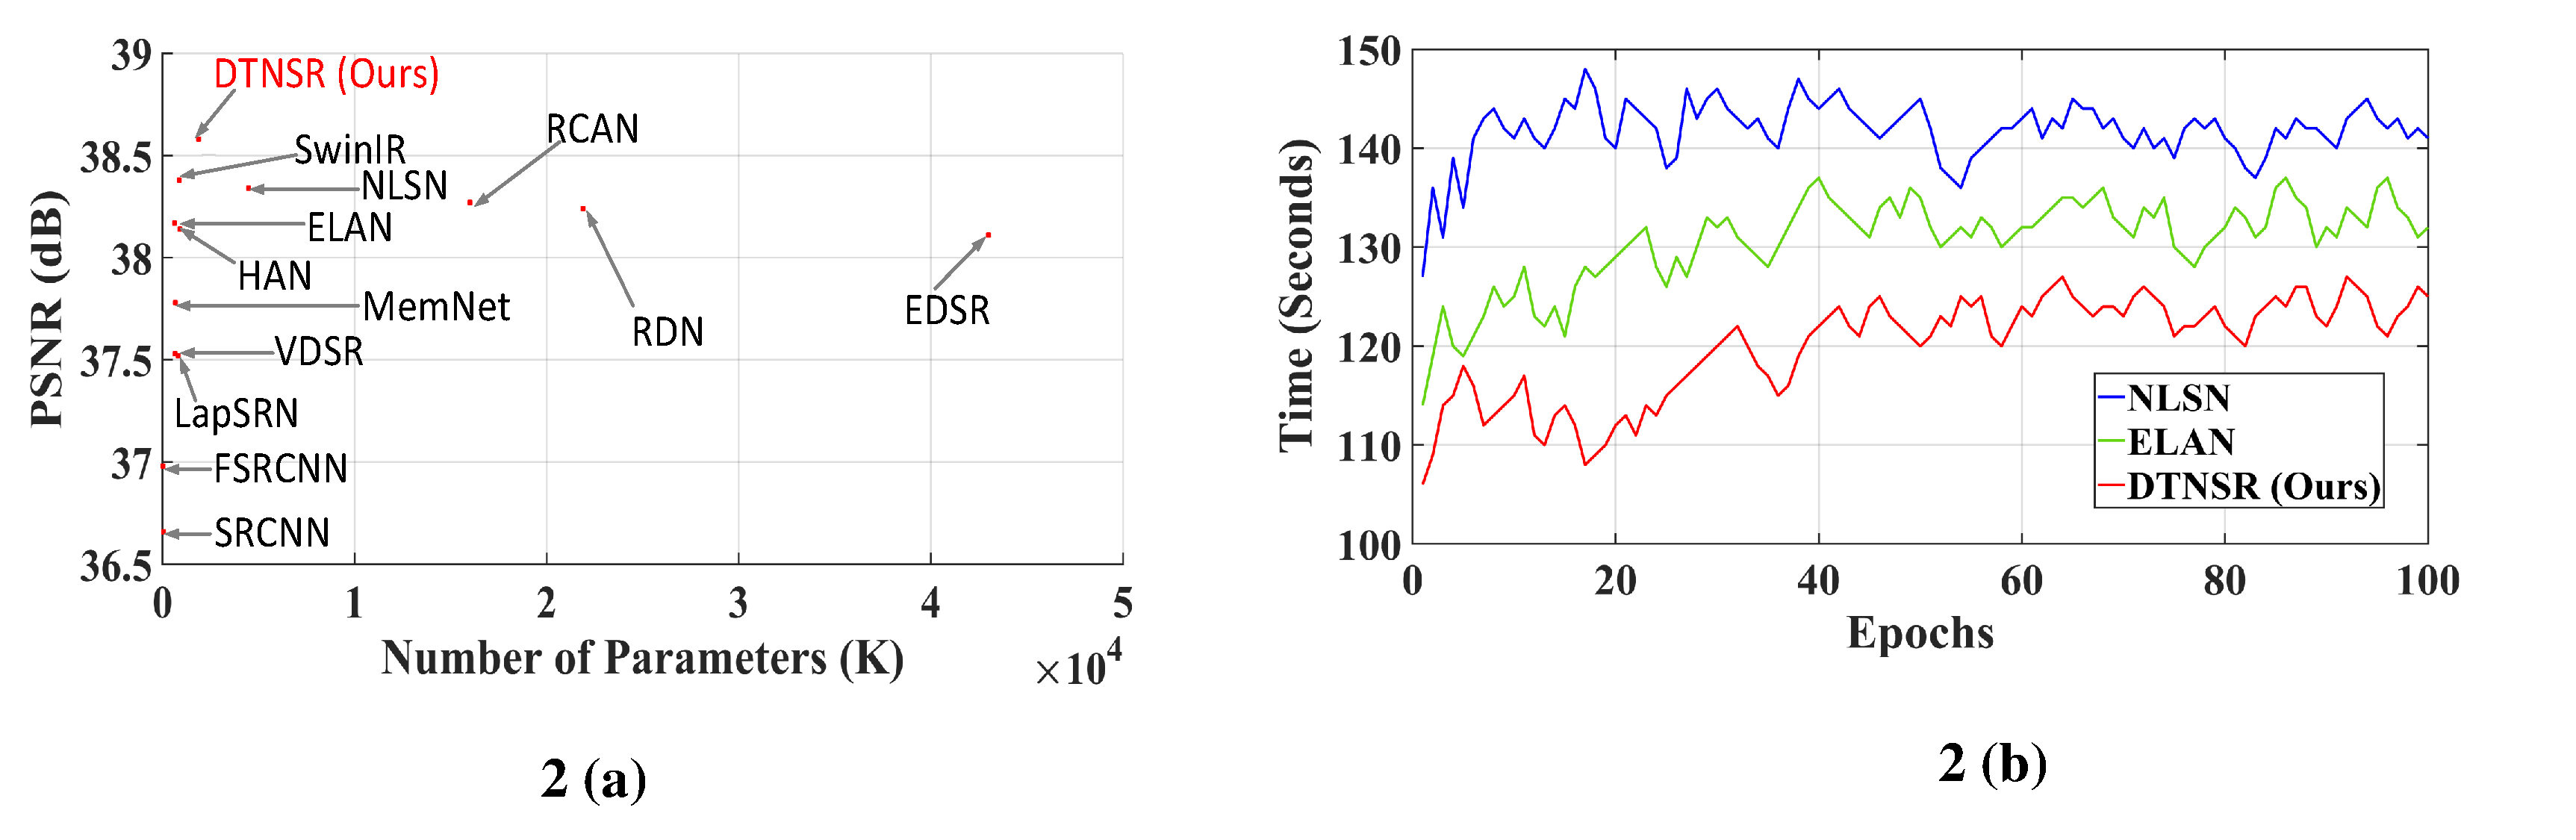
\includegraphics[width=\linewidth]{2FIGURE.pdf}
  \caption{Inspection of PSNR for model parameters on $\times2$ up-scaling factor using the Set5 [37] image test dataset.}
  \label{fig:6}
\end{figure}
\subsection{Perceptual Quality Comparison}
The DTNSR model showcases remarkable fidelity in reducing artifacts and delivering realistic outcomes in Figure 3 and Figure 4. Evaluation at $\times 4$ scale includes the BSD100 [39] dataset's Img\_78004 image, compared against Bicubic, MSRN [44], EDSR [11], AWSRN [42], RCAN [12], NLSN [14], SwinIR [17], and SRFormer [19]. For $\times 8$ scaling, the BSD100 [39] dataset's Img\_302008 image was used, with comparisons made against Bicubic, MSRN [44], DBPN [43], AWSRN [42], RCAN [12], and HAN [15] image SR methods
\begin{multicols}{2}[\columnsep=10pt]
\begin{figure*}
    \includegraphics[width=0.5\linewidth]{3Figure.pdf}
    \caption{Img\_78004 from the BSD100 [40] dataset on $\times4$ up-scaling factor.}
    \label{fig:13}
\end{figure*}

\begin{figure*}
    \includegraphics[width=0.5\linewidth]{4Figure.pdf}
    \caption{Img\_302008 from the BSD100 [40] dataset on $\times8$ up-scaling factor.}
    \label{fig:17}
\end{figure*}
\end{multicols}

\subsection{Ablation assessment}
\subsubsection{Analysis with different window sizes in the Local Feature Window Transformer (LFWT) Block}
To assess the effect of different window sizes we set the window sizes, to be 8 $\times$ 8, 16 $\times$ 16, and 24 $\times$ 24 and Table S1 shows a comparison of our proposed model with existing state-of-the-art transformer-based methods like SwinIR [17] and SRFormer [19] on image SR test dataset for up-scaling factor $\times$ 4. 
\subsubsection{Ablation assessment using traditional denoising methods} 
In this section, we present a comparative analysis of our DTNSR model applied to the Urban100 [41] Dataset at a scale of $\times$2, against traditional denoising approaches including Block Matching and 3D Filtering (BM3D) [46], Fast and Flexible Solution for CNN-Based Image Denoising (FFDNet) [47], Nonlocally Centralized Sparse Representation (NCSR) [48],  and Denoising Convolutional Neural Network (DnCNN) [23]. The evaluation is based on PSNR metrics under Gaussian noise with varying noise levels ($\sigma$), specifically $\sigma = 5$, $\sigma = 10$, and $\sigma = 15$, as summarized in Table S2. 

\section{Conclusions and Future Work}

In conclusion, our work presents the DTNSR model, which combines novel Local Feature Window Transformers with Xception blocks for single-image super-resolution. We effectively handle patches to preserve computational efficiency while guaranteeing accuracy by using a Patch Embedding layer. By combining the LWFT and Xception blocks in a multi-path network backbone, we efficiently balance local and global information. Thus, mitigating over-smoothing and artifact generation. This method also helps to recover noisy images by capturing the hierarchical feature through integrating the Xception Block in the network.The efficacy of the model is demonstrated across a range of up-scaling factors through the evaluation of five benchmark datasets. Future research will focus on refining the model for real-time and high-definition video applications.

\begin{thebibliography}{00}

\bibitem{b1} J. Greenspan, H., \textit{Super-resolution in medical imaging.} The computer journal, 2009. 52(1): p. 43-63.

\bibitem{b2} Lorch, B. and Riess, C., \textit{Image forensics from chroma subsampling of high-quality JPEG images.} In Proceedings of the ACM Workshop on Information Hiding and Multimedia Security. July, 2019. pp. 101-106.

\bibitem{b3} Zhang, Z., Barbary, K., Nothaft, F.A., Sparks, E.R., Zahn, O., Franklin, M.J., Patterson, D.A. and Perlmutter, S.,  \textit{Kira: Processing astronomy imagery using big data technology.} IEEE Transactions on Big Data, 2016. 6(2): pp.369-381.

\bibitem{b4} C. Dong, C. C. Loy, K. He and X. Tang, \textit{"Image super-resolution using deep convolutional networks"}, \textit{IEEE Trans. Pattern Anal. Mach. Intell.}, vol. 38, pp. 295-307, Feb. 2015.

\bibitem{b5} Dong, C., C.C. Loy, and X. Tang. \textit{Accelerating the super-resolution convolutional neural network. in European conference on computer vision}. 2016. Springer.

\bibitem{b6} J. Kim, J. K. Lee and K. M. Lee, \textit{"Accurate image super-resolution using very deep convolutional networks"}, \textit{Proc. IEEE Conf. Comput. Vis. Pattern Recognit.}, pp. 1646-1654, Jun, 2016.

\bibitem{b7} W.-S. Lai, J.-B. Huang, N. Ahuja and M.-H. Yang, \textit{"Deep Laplacian pyramid networks for fast and accurate super-resolution"}, \textit{Proc. IEEE Conf. Comput. Vis. Pattern Recognit.}, pp. 5835-5843, Jul. 2017.

\bibitem{b8} Kim, J., J.K. Lee, and K.M. Lee. \textit{Deeply-recursive convolutional network for image super-resolution}. in \textit{Proceedings of the IEEE conference on computer vision and pattern recognition}. 2016.

\bibitem{b9} Tai, Y., Yang, J. and Liu, X., \textit{Image super-resolution via deep recursive residual network}. In \textit{Proceedings of the IEEE conference on computer vision and pattern recognition}, 2017. (pp. 3147-3155).

\bibitem{b10} Y. Tai, J. Yang, X. Liu and C. Xu, \textit{"MemNet: A persistent memory network for image restoration"}, \textit{Proc. IEEE Conf. Int. Conf. Comput. Vis.}, Oct 2017. pp. 4539-4547. 

\bibitem{b11} Lim, B., \textit{Enhanced deep residual networks for single image super-resolution}. in \textit{Proceedings of the IEEE conference on computer vision and pattern recognition workshops}. 2017.

\bibitem{b12} Zhang, Y., et al. \textit{Image super-resolution using very deep residual channel attention networks}. in \textit{Proceedings of the European conference on computer vision (ECCV)}. 2018.

\bibitem{b13} Mei, Y., et al. \textit{Image super-resolution with cross-scale non-local attention and exhaustive self-exemplars mining}. in \textit{Proceedings of the IEEE/CVF conference on computer vision and pattern recognition}. 2020.

\bibitem{b14} Mei, Y., Y. Fan, and Y. Zhou. \textit{Image super-resolution with non-local sparse attention}. in \textit{Proceedings of the IEEE/CVF Conference on Computer Vision and Pattern Recognition}. 2021.

\bibitem{b15} Niu, B., Wen, W., Ren, W., Zhang, X., Yang, L., Wang, S., Zhang, K., Cao, X. and Shen, H., 2020. \textit{Single image super-resolution via a holistic attention network}. In \textit{Computer Vision–ECCV 2020: 16th European Conference, Glasgow, UK, August 23–28, 2020, Proceedings, Part XII 16} (pp. 191-207). Springer International Publishing.

\bibitem{b16} Zhang, X., Zeng, H., Guo, S. and Zhang, L., \textit{Efficient long-range attention network for image super-resolution.} In European Conference on Computer Vision (pp. 649-667). Cham: Springer Nature Switzerland, Oct, 2022.

\bibitem{b17} Liang, J., Cao, J., Sun, G., Zhang, K., Van Gool, L. and Timofte, R. \textit{SwinIR: Image restoration using swin transformer}. In \textit{Proceedings of the IEEE/CVF international conference on computer vision}, 2021. (pp. 1833-1844).

\bibitem{b18} Liu, Z., Lin, Y., Cao, Y., Hu, H., Wei, Y., Zhang, Z., Lin, S. and Guo, B. \textit{Swin Transformer: Hierarchical vision transformer using shifted windows.} In Proceedings of the IEEE/CVF international conference on computer vision, 2021. (pp. 10012-10022).

\bibitem{b19} Zhou, Y., Li, Z., Guo, C.L., Bai, S., Cheng, M.M. and Hou, Q. \textit{SRFormer: Permuted Self-Attention for Single Image Super-Resolution.} arXiv preprint, 2023. arXiv:2303.09735.

\bibitem{b20} Dosovitskiy A., Beyer L., Kolesnikov A., Weissenborn D., Zhai X., Unterthiner T., Dehghani M., Minderer M., Heigold G., Gelly S., Uszkoreit J., and Houlsby N. \textit{An image is 11worth 16$\times$16 words: Transformers for image recognition at scale.} In International Conference on Learning Representations, 2021.

\bibitem{b21} Chollet, F. \textit{Xception: Deep learning with depthwise separable convolutions.} In Proceedings of the IEEE Conference on Computer Vision and Pattern Recognition (pp. 1251-1258). 2017.

\bibitem{b22} Mehri, A., Ardakani, P.B. and Sappa, A.D. \textit{MPRNet: Multi-path residual network for lightweight image super-resolution.} In Proceedings of the IEEE/CVF Winter Conference on Applications of Computer Vision, 2021. pp. 2704-2713.

\bibitem{b23} Chen, J. and Li, F., \textit{Denoising convolutional neural network with mask for salt and pepper noise}. IET Image Processing, 2019. 13(13), pp.2604-2613.

\bibitem{b24} K.-W. Hung, Z. Zhang and J. Jiang, \textit{"Real-time image super-resolution using recursive depthwise separable convolution network"}, \textit{IEEE Access}, vol. 7, 2019. pp. 99804-99816.

\bibitem{b25} X. Yang, H. Mei, J. Zhang, K. Xu, B. Yin, Q. Zhang, et al., \textit{"DRFN: Deep recurrent fusion network for single-image super-resolution with large factors"}, \textit{IEEE Trans. Multimedia}, Feb. 2019. vol. 21, no. 2, pp. 328-337.

\bibitem{b26} Wazir M., Aramvith S., and Onoye T. \textit{"SENext: Squeeze-and-ExcitationNext for Single Image Super-Resolution." }IEEE Access (2023).

\bibitem{b27} K. Zhang, W. Zuo and L. Zhang, \textit{"Learning a single convolutional super-resolution network for multiple degradations}", \textit{Proc. IEEE/CVF Conf. Comput. Vis. Pattern Recognit.}, Jun. 2018. vol. 6, no. 1, pp. 3262-3271.

\bibitem{b28} C. Ledig, L. Theis, F. Huszar, J. Caballero, A. Cunningham, A. Acosta, A. P. Aitken, A. Tejani, J. Totz, Z. Wang et al., \textit{Photorealistic single image super-resolution using a generative adversarial network} in CVPR, 2017.

\bibitem{b29} X. Wang, K. Yu, S. Wu, J. Gu, Y. Liu, C. Dong, C. C. Loy, Y. Qiao, and X. Tang, \textit{Esrgan: Enhanced super-resolution generative adversarial networks} in ECCV Workshop, 2018.

\bibitem{b30} Zhang, Y., et al. \textit{Residual dense network for image super-resolution}. in \textit{Proceedings of the IEEE conference on computer vision and pattern recognition}. 2018.

\bibitem{b31} Ruangsang W., Aramvith S., and Onoye T. "Multi-FusNet of Cross Channel Network for Image Super-Resolution." IEEE Access (2023).

\bibitem{b32} Talreja, J., Aramvith, S. and Onoye, T. \textit{DANS: Deep Attention Network for Single Image Super-Resolution.} IEEE Access, 2023.

\bibitem{b33} Wolf, T., Debut, L., Sanh, V., Chaumond, J., Delangue, C., Moi, A., Cistac, P., Rault, T., Louf, R., Funtowicz, M. and Davison, J. \textit{Transformers: State-of-the-art natural language processing.} In Proceedings of the 2020 conference on empirical methods in natural language processing: system demonstrations, October 2020. pp. 38-45.

\bibitem{b34} Taud, H. and Mas, J.F. \textit{Multilayer perceptron (MLP).} Geomatic approaches for modeling land change scenarios, 2018.  pp.451-455.

\bibitem{b35} Arora, R., Basu, A., Mianjy, P. and Mukherjee, A. \textit{Understanding deep neural networks with rectified linear units.} arXiv preprint, 2016. arXiv:1611.01491.

\bibitem{b36} Agustsson, E.,  Timofte, R. \textit{"NTIRE 2017 Challenge on Single Image Super-Resolution: Dataset and Study."} IEEE Conference on Computer Vision and Pattern Recognition Workshops (CVPRW), (2017). 126-135.

\bibitem{b37} Bevilacqua, M.; Roumy, A.; Guillemot, C.; Alberi-Morel, M.L. \textit{Low-complexity single-image super-resolution based on nonnegative neighbor embedding}. In \textit{Proceedings of the British Machine Vision Conference, Surrey}, UK, 3–7 September 2012.

\bibitem{b38} Zeyde, R.; Elad, M.; Protter, M. \textit{On Single Image Scale-Up Using Sparse-Representations}. In \textit{Proceedings of the International Conference on Curves and Surfaces}, Oslo, Norway, 28 June–3 July 2012; pp. 711–730.

\bibitem{b39} Martin, D.; Fowlkes, C.; Tal, D.; Malik, J. \textit{A database of human segmented natural images and its application to evaluating segmentation algorithms and measuring ecological statistics}. In \textit{Proceedings of the Eighth International Conference On Computer Vision} (ICCV-01), Vancouver, BC, Canada, 7–14 July 2001.

\bibitem{b40} Huang, J.-B.; Singh, A.; Ahuja, N. \textit{Single image super-resolution from transformed self-exemplars}. In \textit{Proceedings of the IEEE Conference on Computer Vision and Pattern Recognition}, Boston, MA, USA, 7–12 June 2015.

\bibitem{b41} Matsui, Y.; Ito, K.; Aramaki, Y.; Fujimoto, A.; Ogawa, T.; Yamasaki, T.; Aizawa, K. \textit{Sketch-based manga retrieval using manga109 dataset}. Multimedia. Tools Appl. 2017, 76, 21811–21838.

\bibitem{b42} Wang, C., Li, Z. and Shi, J., \textit{Lightweight image super-resolution with adaptive weighted learning network}, 2019. arXiv preprint arXiv:1904.02

\bibitem{b43} Haris, M., Shakhnarovich, G. and Ukita, N. \textit{Deep back-projection networks for super-resolution.} In Proceedings of the IEEE conference on computer vision and pattern recognition, 2018. pp. 1664-1673.

\bibitem{b44} J. Li, F. Fang, K. Mei and G. Zhang, \textit{"Multi-scale residual network for image super-resolution"}, \textit{Proc. Eur. Conf. Comput. Vis. (ECCV)}, Sep 2018. pp. 517-532.

\bibitem{b45} Dabov, K., Foi, A., Katkovnik, V. and Egiazarian, K. \textit{Color image denoising via sparse 3D collaborative filtering with grouping constraint in luminance-chrominance space.} In 2007 IEEE international conference on image processing, September 2007. (Vol. 1, pp. I-313). IEEE.

\bibitem{b46} Zhang, K., Zuo, W. and Zhang, L., 2018. \textit{FFDNet: Toward a fast and flexible solution for CNN-based image denoising.} IEEE Transactions on Image Processing, 27(9), pp.4608-4622.

\bibitem{b47} Dong, W., Zhang, L., Shi, G. and Li, X. \textit{Nonlocally centralized sparse representation for image restoration.} IEEE Transactions on Image Processing, 22(4),  2012. pp.1620-1630.

\end{thebibliography}

\end{document}
